Laikā kodētos impulsu signālus no \Gls{aer} dekodētāja apstrādā uz notikumiem balstītu konvolūciju slāņi, kā ilustrēts \ref{fig:bsf_arch}.
attēlā. Šie slāņi atdarina sinaptiskās operācijas fiksētā uztveres laukā, veicot ieejas impulsu svērto summēšanu, kā
aprakstīts (\ref{eq:channel_conv}). Tā kā impulsi ir bināri ($s \in \{0,1\}$), apstrādes kodols tradicionālās \Gls{mac}
operācijas starp datiem un svariem aizstāj ar svaru bināro maskēšanu, reducējot impulsa un svara reizināšanu līdz
\begin{equation}
  w \cdot s =
  \begin{cases}
    w, & s=1 \\
    0, & s=0
  \end{cases}
\end{equation}
Tas ļauj reizināšanas operāciju aizstāt ar nosacītu svara izvēli. Tai seko \Gls{acc}, kas realizēta ar \Gls{pta}. Būtiski, ka šīs \Gls{acc} operācijas vada notikumi un tās notiek tikai tad, ja ir impulsi, ievērojami samazinot liekus aprēķinus.

Šajā shēmā svaru un nobīžu parametri tiek glabāti divportu \Gls{ocm} blokos tuvu apstrādes loģikai. Šī pieeja izmanto FPGA iekšējo \Gls{bram}, lai samazinātu latentumu un izvairītos no ārējās atmiņas transakcijām. Svari tiek statiski konfigurēti pirms izpildes ar atmiņā kartētu AXI-Lite saskarni un atkārtoti izmantoti katrā inferences ciklā. Lai gan dziļajiem SNN var būt nepieciešams ievērojams svaru atmiņas apjoms, svaru bitu platuma kvantēšanu var piemērot, nemazinot veiktspēju \cite{shen2024}.

\begin{figure}[htbp]
  % 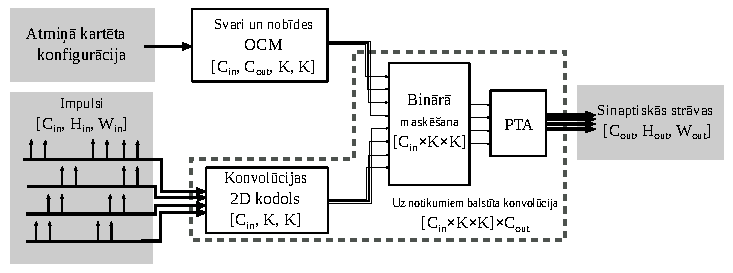
\includegraphics[width=\columnwidth]{fig/lv/conv_layer-v1.pdf}
  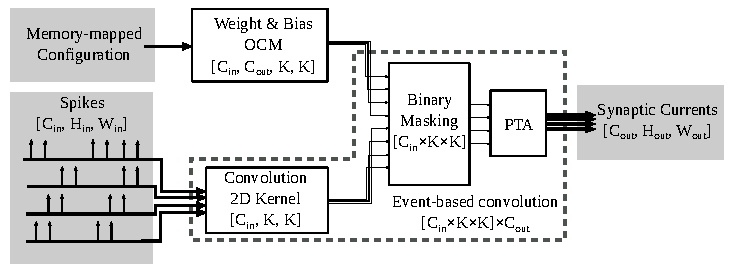
\includegraphics[width=\columnwidth]{fig/conv_layer-v1.pdf}
  \caption{Binārs telpiskais filtrs ar uz notikumiem balstītām konvolūcijām.}
  \label{fig:bsf_arch}
\end{figure}

Konvolūcijas 2D kodols savāc \(K \times K\) telpisko logu no katra ieejas impulsu pazīmju kartes kanāla \(C_{in}\). Impulsi tiek straumēti pa AXI-Stream saskarni uz binārās maskēšanas bloku, savukārt svariem izmanto otru straumēšanas saskarni.

Resursu taupīšanai maskēšanas un \Gls{pta} operācijas tiek veiktas secīgi katram ieejas kanālam \([C_{in}, K, K]\) kodolā un multipleksētas laikā starp \(C_{out}\) izejas kanāliem, kā parādīts \ref{fig:conv_steps}. attēlā. Tas ļauj atkārtoti izmantot to pašu apstrādes loģiku, būtiski samazinot nepieciešamo aparatūras resursu apjomu. Lai samazinātu izpildes laiku, laikā multipleksētā loģika netiek darbināta neaktīvajos laika soļos, izvairoties no nevajadzīgiem aprēķiniem, ja nav ieejas impulsu.

\begin{figure}[htbp]
  % 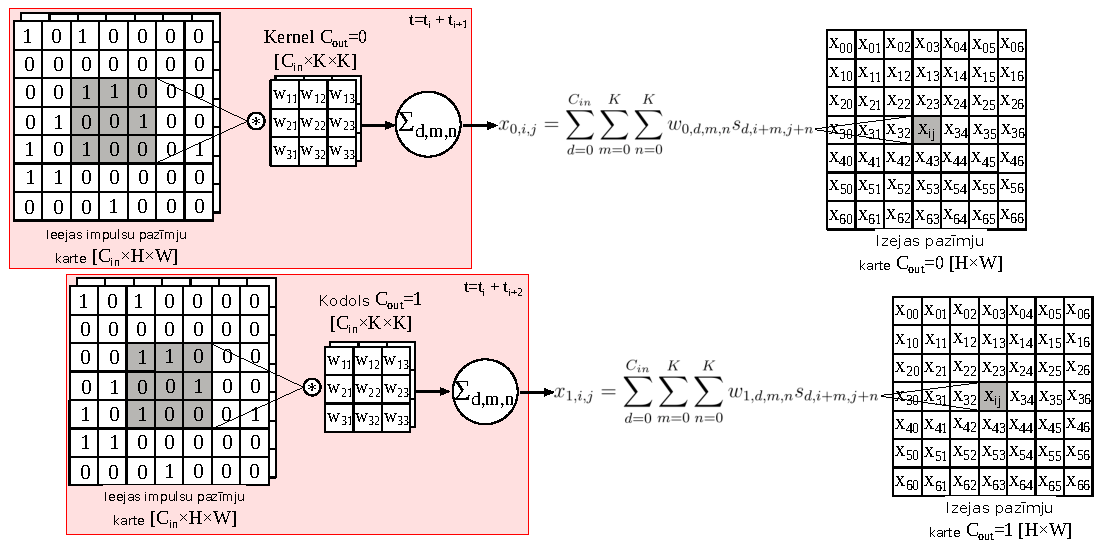
\includegraphics[width=\columnwidth]{fig/lv/conv_time_steps-v2.pdf}
  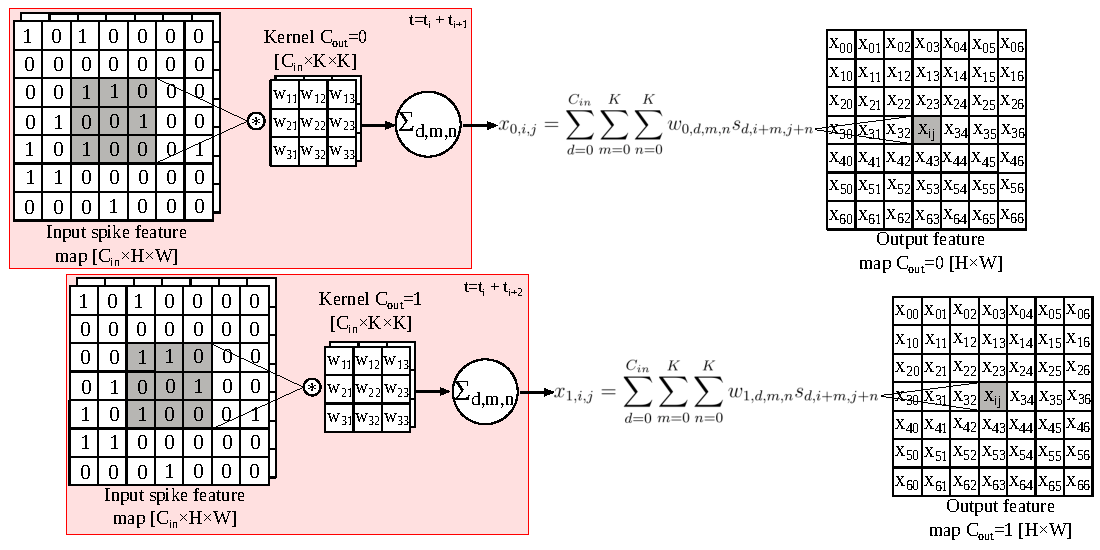
\includegraphics[width=\columnwidth]{fig/conv_time_steps-v2.pdf}
  \caption{Retināta konvolūcija ar līdzsvarotu paralēlismu un resursu atkārtotu izmantošanu: paralēla ieejas kanālu apstrāde un laikā multipleksēta izejas kanālu apstrāde.}
  \label{fig:conv_steps}
\end{figure}

Konvolūcijas soli, kanālu skaitu un ieejas attēla izmērus izpildes laikā var pārkonfigurēt ar īpašiem konfigurācijas reģistriem, novēršot atkārtotas sintēzes nepieciešamību.

Šī moduļa izeja ir sinaptiskās strāvas vektors ar \(C_{out}\) izejas kanāliem, kas pēc tam kalpo par ieeju nākamajiem \Gls{lif} integrēšanas un sliekšņa salīdzināšanas blokiem.


